\section{Tidsplan}
\label{bilag1}
\begin{figure}[H]
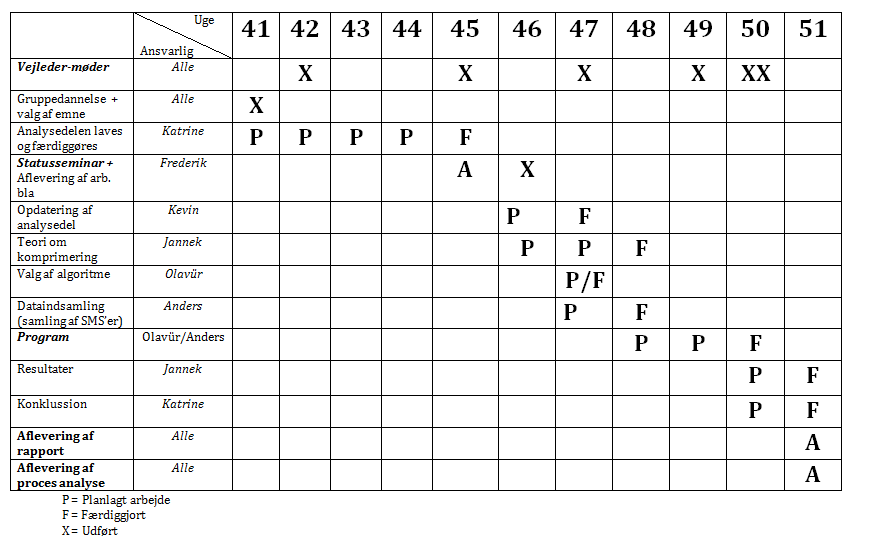
\includegraphics[width=\textwidth]{Indhold/tidsplan.png}
\caption {Tidsplanen for projektet}
\label {tidsplan}
\end{figure}

\section{Arbejdsintensitet på GitHub}
\label{bilag2}
\begin{figure}[H]
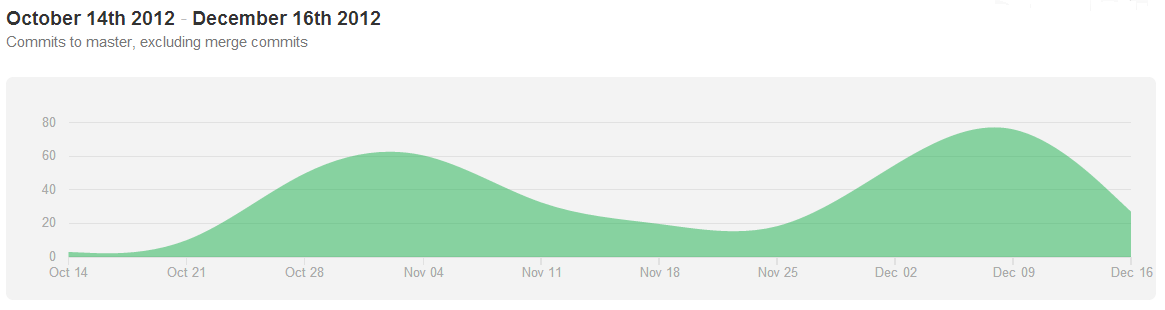
\includegraphics[width=\textwidth]{Indhold/arbejdsintensitet.png}
\caption {Billedet viser hvor ofte vi har "commitet" nye filer eller nyt arbejde til vores fælles mappe}
\label {arbejde}
\end{figure}


\section{Eksempel på referat fra vejledermøde}

Ok, at bruge kilder hvis ingen bedre findes.

Forklaring af kode:
Kun forklaring af de større beslutningsmæssige trin.
Ikke bruge en side på hver funktion, men det er en god ide at uddybe nogle enkelte funktioner som er vigtige
Nogen vedlægger en cd med program. Andre lægger kildekode som appendiks. Github kan evt godt bruges.

Programmerings delen er fuldt i gang, med mere end 1000 linjers kode skrevet.

Inkludere dynamisk træ, for at se forskellen.
Ved et dynamisk træ kan træet være betydeligt mindre end et statisk træ, da tegnene vil være færre

God ide at se på wikipedias træ vs sms træ. (Husk at fjerne specielle tegn fra wiki).

Caption på billeder, der mangler
Scalering af figurer.

Eksamens information:
Guide kommer snart (færdig i weekenden)
Alle skal helst snakke lige meget.
Prøvefremlæggelser. (med tidstagning)
Afsat 58 minutter til fremlæggelse.
Rikke er ikke med i gruppen.
Byd ind når muligheden byder sig. Jo mere der siges ved den fælles del, jo nemmere vil det være ved spørgsmål.

5 min per student til karaktergivning.
Karakter gives fælles.

3 timer og 30 minutter afsat.

Alt skal være klart (projektor etc.) før fremlæggelsen.

Efter fremlæggelse lades pc være tændt.
Hav alt på pc'en.

Navneskilte

powerpoint eller bima eller google docs

Fremlæggelsen må meget gerne gå ud over rapporten. Det er projektet som fremlægges ikke rapporten.

Af hensyn til bivejleder og censor, kan det være godt at finde måder hvor der ikke tales direkte om programmet.

Der må gerne lave rettelsesblade før fremlæggelsen, og er en rigtig god idé, da det viser at vi selv allerede har fundet fejl i rapporten. Kun hvis man selv finder fejl. Afleveres til eksamen.

Udprintet slides kan være en god idé, men der er delte meninger om dette emne. (Skader ikke).

Det er en god idé at lave en introduktion til afsnittet, og en opsummering til sidst.
Afsnitskonklusion kan være vigtigt, men ikke i alle sammenhænge.

Lærer og censor har læst og klargjort spørgsmål til rapporten.
De kan stille spørgsmål hvis de ikke har forstået en del af rapporten.

Næste møde:
Hvis vi vil holde møde mandag formiddag, skal vi kontakte Michael fredag morgen, og sende rapporten senest klokken 6.
Det er også muligt at holde mail møde, ved at sende rapporten i løbet af weekenden.